\section{Limterms, LIM rewrites}
\label{emr}


The main idea of emergent algebras  is to allow the "passage to the limit" of the node variables, in some cases. This requires the enlargement of the class of constant terms, and the introduction of limterms. 

\begin{definition}
We add to the class of constant terms the ("exact") sum $\displaystyle \Sigma_{0}$,  the ("exact") diff $\displaystyle \Delta_{0}$, the ("exact") inv $\displaystyle inv_{0}$. 

We define the class of limterms as: 
\begin{enumerate}
\item[-] any term is a limterm. If $b$ is a term then the set of free node variables of $b$ is defined by $\displaystyle Freenodevar(b) \, = \, Nodevar(b)$ and the set of bonded node variables is  $Bondnodevar(b) \, = \, \emptyset$.
\item[-] if $a \in \Upsilon$ and $b$ is a limterm  then $\displaystyle L a. b$ is a limterm, with $\displaystyle Freenodevar(La.b) \, = \, Freenodevar(b) \setminus \left\{ a \right\}$ and $Bondnodevar(La.b) \, = \, Bondnodevar(b) \cup \left\{ a \right\}$.
\item[-] if $t$ is a limterm and $\displaystyle \in \Upsilon \cup \left\{ 0,1 \right\}$ then $t b$ is a limterm, with $\displaystyle Freenodevar(t b) \, = \, Freenodevar(t)$ and $\displaystyle Bondnodevar(t b) \, = \, Bondnodevar(t)$. 

The alpha renaming is extended to limterms. 
\end{enumerate}
\end{definition}

\begin{figure}[h]\centerline{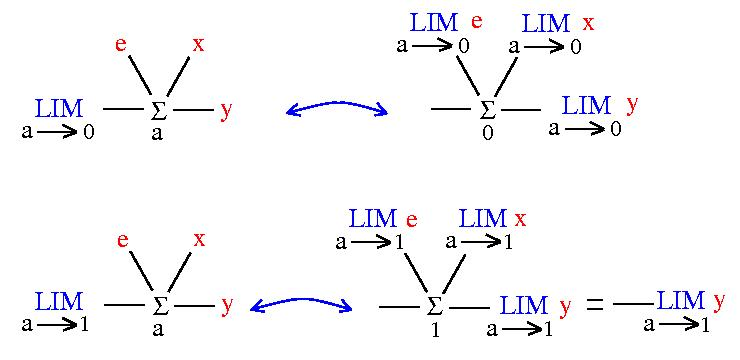
\includegraphics[width=120mm]{jpg/asum-em-alt.jpg}}  \caption{ The graphical notation for the LIM rewrite for the sum term} \label{asum-em-alt-fig} \end{figure}

\begin{definition}
The LIM rewrites are: 
\begin{enumerate}
\item[-] the LIM rewrites for edge variables: if $e$ is an edge variable, $a \in \Upsilon$ and $\displaystyle b \in \Upsilon \cup \left\{ 0 , 1 \right\}$, then $$(La.e)b \, \stackrel{LIM}{\longleftrightarrow} \, e$$  
\item[-] the LIM rewrites for node variable limterms: if $e, x$ are limterms then 
$$\displaystyle \left(La.\left(a^{e} x\right)\right) b  \, \stackrel{LIM}{\longleftrightarrow} \, b^{(La.e)b} (La.x)b$$ for $\displaystyle b \in \Upsilon \cup \left\{ 0 , 1 \right\}$, and  
$$\displaystyle \left(La.\left(\bar{a}^{e} x\right)\right) b  \, \stackrel{LIM}{\longleftrightarrow} \, \bar{b}^{(La.e)b} (La.x)b$$ for $\displaystyle b \in \Upsilon \cup \left\{  1 \right\}$. 
\item[-] the LIM rewrite for the sum term: if $e, x, y$ are limterms then 
$$\displaystyle \left( La.\Sigma_{a}^{e}(x,y) \right) b \, \stackrel{LIM}{\longleftrightarrow} \, \Sigma_{b}^{(La.e)b}((La.x)b,(La.y)b)$$ for $\displaystyle b \in \Upsilon \cup \left\{ 0 , 1 \right\}$. 
The term $\displaystyle \Sigma_{1}^{e} (x,y) \, = \, y$ is obtained from the application of the LIM rewrites for node variable terms to the limterm $\displaystyle (La.\Sigma_{a}^{e}(x,y)) 1$. 
\item[-] the LIM rewrite for the diff term: if $e, x, y$ are limterms then $$\displaystyle \left( La.\Delta_{a}^{e}(x,y)\right)b \, \stackrel{LIM}{\longleftrightarrow} \, \Delta_{b}^{(La.e)b}((La.x)b,(La.y)b)$$ for $\displaystyle b \in \Upsilon \cup \left\{ 0 , 1 \right\}$. 
The term $\displaystyle \Delta_{1}^{e} (x,y) \, = \, y$ is obtained from the application of the LIM rewrites for node variable terms to the term $\displaystyle (La.\Delta_{a}^{e}(x,y)) 1$. 
\item[-] the LIM rewrite for the inv term: $$\displaystyle \left(La.inv_{a}^{e} x\right) \, \stackrel{LIM}{\longleftrightarrow} \, inv_{0}^{(La.e)b} (La.x)b$$ for $\displaystyle b \in \Upsilon \cup \left\{ 0 , 1 \right\}$. The term $\displaystyle inv_{1}^{e} x  \, = \, e$ is obtained from the application of the LIM rewrites for node variable terms to the limterm $\displaystyle (La,inv_{a}^{e} x) 1$. 
\end{enumerate}

\end{definition}
